\documentclass[captions=tableheading]{scrartcl}

\usepackage{amsmath}
\usepackage{amssymb}
\usepackage[utf8]{inputenc}
\usepackage[T1]{fontenc}
\usepackage{lmodern}
\usepackage{ngerman}
\usepackage{geometry}
\usepackage{graphicx}
\usepackage{wrapfig}
\usepackage{caption}
\usepackage{wasysym}
\usepackage[separate-uncertainty=true]{siunitx}
\usepackage{picinpar}
\usepackage{tikz}
\usepackage{float}
\usepackage{booktabs}
\usepackage{enumitem} 

\renewcommand{\figurename}{Abb.}
\usepackage[
	colorlinks=true,
	urlcolor=blue,
	linkcolor=black
]{hyperref}

\sisetup{tophrase={{\,\,bis\,\,}}}

%Hier Titel und so
\newcommand{\versuchnummer}{} 
\newcommand{\versuchname}{Röntgenreflektometrie} 
\newcommand{\versuchdatum}{16.02.2017} 
\newcommand{\im}{\mathrm{i}}
\newcommand{\indx}[1]{\text{#1}}
\newcommand{\RE}[1]{\mathrm{Re} \left(#1 \right)}


\title{Versuch \versuchnummer\\ \versuchname}
\subtitle{Physikalisches Fortgeschrittenenpraktikum}
\author{Robert Rauter und Björn Lindhauer}
\date{\versuchdatum} 
\begin{document}
\begin{titlepage}
{\large \versuchdatum}
\vspace{7cm}
\begin{center}
\textbf{\huge \versuchname}\\
\vspace{0.2cm}
\textbf{Physikalisches Fortgeschrittenenpraktikum}\\
\vspace{9cm}

{\Large Robert Rauter \ \ \hspace{1.5cm} und \hspace{1.5cm} Björn Lindhauer}\\
{ \url{robert.rauter@tu-dortmund.de} \ \ \hspace{2cm} \url{bjoern.lindhauer@tu-dortmund.de}}
\end{center}
\end{titlepage}

\section{Theoretische Grundlagen}
Bei der Röntgenreflektometrie werden elektromagnetische Wellen mit Wellenlänge \\ 
$\lambda=$ \SIrange{0.1}{10}{\angstrom} und dem Feldvektor 
\begin{equation}
E\left(r\right)=E_0 \exp\left(\im  k\cdot r \right)
\end{equation}
betrachtet, die aus dem Vakuum mit Brechungsindex $n_1=1$ auf ein Medium mit Brechungsindex $n_2:=n \neq 1$ treffen.

Bei Röntgenstrahlen ist der Realteil des Brechungsindex $n$ geringfügig kleiner als 1, da die Schwingungsfrequenz von Röntgenstrahlung höher ist als die Resonanzfrequenz von Elektronen in einem Medium.
Ist der Realteil des Brechungsindex kleiner als eins, so ist die Phasengeschwindigkeit größer als die Lichtgeschwindigkeit $c$.
Dies ist kein Widerspruch zur Relativitätstheorie, da die relavante Geschwindigkeit für Informationsaustausch die Gruppengeschwindigkeit ist und diese unter der Lichtgeschwindigkeit liegt.

Weil der Brechungsindex nahe Eins liegt, wird er häufig als
\begin{equation}
n=1-\delta + \im\beta \hspace{0.5cm}\text{,}\hspace{0.1cm} \delta >0
\end{equation}
geschrieben. 
Die Korrektur $\delta$ liegt in der Größenordnung $10^{-6}$ und beschreibt die Dispersion. 
Die Absorption wird durch den Parameter $\beta$ beschrieben und liegt für Röntgenstrahlen der Energie $E=$\SI{8}{\kilo\eV} bei $\beta \sim 10^{-7}$.

\subsection{Einschichtsystem}
In diesen Abschnitt wird zunächst die Reflexion der Röntgenstrahlen an einer homogenen Schicht betrachtet.
Die elektromagnetische Welle trifft auf die Oberfläche der homogenen Schicht und wird, wie in Abbildung \ref{fig:reflexionschicht} dargestellt, teilweise reflektiert und teilweise gebrochen.
\begin{center}
	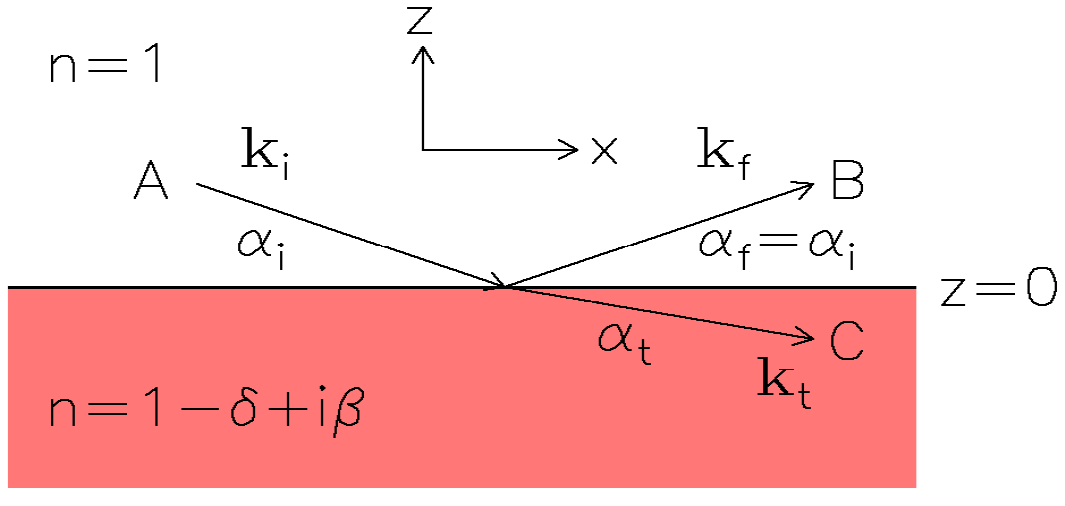
\includegraphics[width=10cm]{images/reflexionschicht.png}
	\captionof{figure}{Graphische Darstellung der einfallenden, reflektierten und gebrochenen Strahlen an einer Grenzschicht mit unterschiedlichen Brechungsindex. \ref{q:anleitung}}
	\label{fig:reflexionschicht}
\end{center}
Es kann in diesen Fall das Brechungsgesetz nach Snellius angewendet werden, nur ist zu beachten, dass die Winkel aufgrund ihrer kleinen Größe im Bezug zur Oberfläche und nicht im Bezug auf das Lot gemessen werden. 
Dies führt zu einer Phasenverschiebung von $\frac{\pi}{2}$ in den trigonometrischen Funktionen.
Somit lautet das Brechungsgesetz nach Snellius
\begin{equation}
\cos \alpha_{\indx{i}}=n\cos \alpha_{\indx{t}} \hspace{0.5cm}\text{.}
\end{equation}
Dies hat zur Folge, dass aufgrund von $\RE{n}<1 $ ein kritischer Winkel
\begin{equation}
\alpha_{\indx{c}}=\arccos n \approx \sqrt{2\delta } = \lambda \sqrt{\frac{r_{\indx{e}} \rho}{\pi}}
\label{eq:elektronendichte}
\end{equation}
existiert, und ab $\alpha \le \alpha_{\indx{c}}$ nur noch Totalreflexion auftritt.
Dabei ist $\lambda$ die Wellenlänge der Röntgenstrahlung, $r_{\indx{e}}$ der klassische Elektronenradius und $\rho$ die Elektronendichte des Materials. 

Wie in der Optik gelten die Fresnelformeln für s-polarisierte Strahlung
\begin{equation}
r_{\indx{s}}= \frac{B}{A}= \frac{k_{\indx{i}}^{\left(z\right)}-k_{\indx{t}}^{\left(z\right)}}{k_{\indx{i}}^{\left(z\right)}+k_{\indx{t}}^{\left(z\right)}}
\end{equation}
\begin{equation}
t_{\indx{s}}= \frac{C}{A}= \frac{2k_{\indx{i}}^{\left(z\right)}}{k_{\indx{i}}^{\left(z\right)}+k_{\indx{t}}^{\left(z\right)}}
\end{equation}
und für die p-polarisierte Strahlung 
\begin{equation}
r_{\indx{p}}= \frac{B}{A}= \frac{n^2 k_{\indx{i}}^{\left(z\right)}- k_{\indx{t}}^{\left(z\right)}}{k_{\indx{i}}^{\left(z\right)}+k_{\indx{t}}^{\left(z\right)}}
\end{equation}
\begin{equation}
t_{\indx{p}}= \frac{C}{A}= \frac{2nk_{\indx{i}}^{\left(z\right)}}{n^2k_{\indx{i}}^{\left(z\right)}+k_{\indx{t}}^{\left(z\right)}}
\end{equation}
mit $k_{\indx{i}}^{\left(z\right)}=k\sin \alpha_{\indx{i}}$ der z-Koordinate der einfallenden Welle und $k_{\indx{t}}^{\left(z\right)}=nk\sin \alpha_{\indx{t}}$ der z-Koordinate der transmittierten Welle.

Da für Röntgenstrahlen der Brechungsindex $n\approx 1$ ist, kann ein gemeinsamer Transmissions- und Reflexionskoeffizient 
\begin{equation}
r= \frac{B}{A}= \frac{k_{\indx{i}}^{\left(z\right)}- k_{\indx{t}}^{\left(z\right)}}{k_{\indx{i}}^{\left(z\right)}+k_{\indx{t}}^{\left(z\right)}}
\end{equation}
\begin{equation}
t= \frac{C}{A}= \frac{2k_{\indx{i}}^{\left(z\right)}}{k_{\indx{i}}^{\left(z\right)}+k_{\indx{t}}^{\left(z\right)}}
\end{equation}
für s- und p-polarisierte Strahlung verwendet werden. 

Die messbare Intensität ist durch
\begin{equation}
R_{\indx{F}  }=\frac{I_{\indx{R}}}{I_{\indx{0}}}= \left\vert r \right\vert^2
\end{equation}
gegeben.
Wird der Einfallwinkel der Röntgenstrahlung so gewählt, dass $\alpha_{\indx{i}}>3\alpha_{\indx{c}}$ ist, so ist $R_{\indx{F}  }$ näherungsweise durch
\begin{align}
R_{\indx{F}}&=\left\vert r \right\vert^2=\left( \frac{k\sin \alpha_{\indx{i}}  - k\sqrt{ \cos^2 \alpha_{\indx{c}} - \cos^2 \alpha_{\indx{i}} }}{k\sin \alpha_{\indx{i}}  + k\sqrt{ \cos^2 \alpha_{\indx{c}} - \cos^2 \alpha_{\indx{i}} }}  \right)^2\\
&\approx \left( \frac{\alpha_{\indx{i}}-\sqrt{1-\alpha_{\indx{c}}^2 -1 + \alpha_{\indx{i}}^2} }{\alpha_{\indx{i}}+\sqrt{1-\alpha_{\indx{c}}^2 -1 + \alpha_{\indx{i}}^2}}  \right)^2=\left( \frac{1-\sqrt{ 1 -\left(\frac{\alpha_{\indx{c}} }{\alpha_{\indx{i}}}\right)^2}  }{1+\sqrt{ 1 -\left(\frac{\alpha_{\indx{c}} }{\alpha_{\indx{i}}}\right)^2} }  \right)^2\\
&\approx \left( \frac{1-1+\frac{1}{2}\left(\frac{\alpha_{\indx{c}} }{\alpha_{\indx{i}}}\right)^2 }{1+1-\frac{1}{2}\left(\frac{\alpha_{\indx{c}} }{\alpha_{\indx{i}}}\right)^2}  \right)^2= \left(\frac{\left(\frac{\alpha_{\indx{c}} }{\alpha_{\indx{i}}}\right)^2}{4-\left(\frac{\alpha_{\indx{c}} }{\alpha_{\indx{i}}}\right)^2} \right)^2\approx \left(\frac{1}{4}\left(\frac{\alpha_{\indx{c}} }{\alpha_{\indx{i}}}\right)^2   \right)^2\\
&= \left(\frac{\alpha_{\indx{c}} }{2\alpha_{\indx{i}}}\right)^4
\end{align}
gegeben.
\subsection{Mehrschichtsystem}
Durch Interferenz von Strahlen, die in unterschiedlichen Schichten reflektiert wurden, entstehen bei Mehrschichtsystemen Modulationen, die sogenannten Kiessig-Ringe.
Ist der Gangunterschied ein Vielfaches der halben Wellenlänge, so entsteht ein Interferenzmimimum. 
Bei einer Schichtdicke von $d$ gilt
\begin{equation}
2d\sin \alpha_{\indx{i}} =n\lambda
\end{equation}
\begin{equation}
d=\frac{2\pi}{\Delta q}\approx \frac{\lambda}{2\Delta\alpha_{\indx{i}}}\text{,}
\label{eq:schichtdicke}
\end{equation}
mit $q=2k\sin \alpha_{\indx{i}}$ der Wellenübertrag in z-Richtung. In Abbildung \ref{fig:reflexionschichten} ist dies illustriert.
\begin{center}
	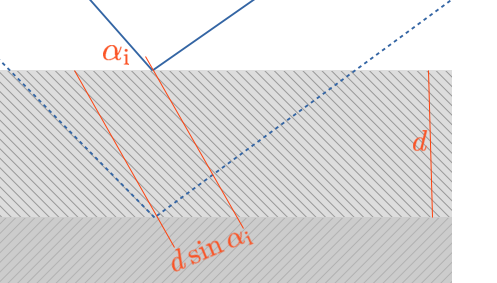
\includegraphics[width=10cm]{images/reflexionschichten.png}
	\captionof{figure}{Schematische Darstellung der destruktiven Interferenz an einem Zweischichtsystem.}
	\label{fig:reflexionschichten}
\end{center}
\begin{center}
	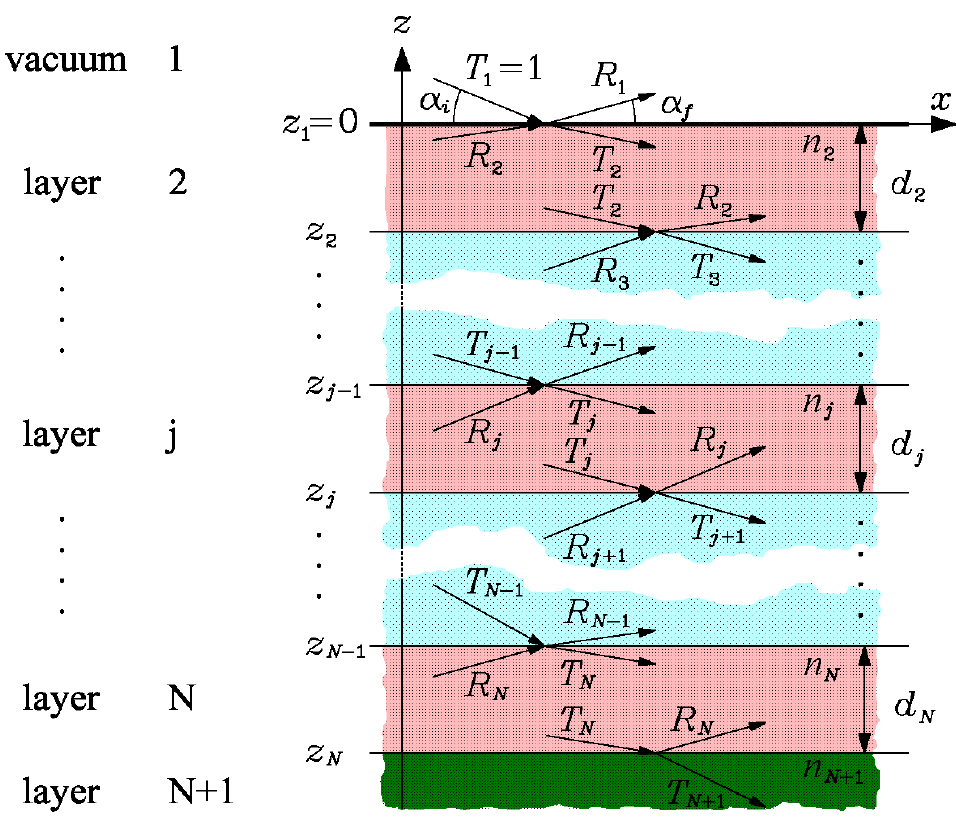
\includegraphics[width=10cm]{images/reflexionmehrschichten.png}
	\captionof{figure}{Schematische Darstellung der Reflexion und Transmission von Röntgenstrahlung
aus dem Vakuum an einem Mehrschichtsystem.  \ref{q:anleitung}}
	\label{fig:reflexionmehrschichten}
\end{center}
Für ein System mit $N$ Schichten, wie in Abbildung \ref{fig:reflexionmehrschichten} dargestellt, kann die Röntgenreflektivität durch den Parratt-Algorithmus berechnet werden. 
Dieser berechnet rekursiv das Verhältnis der reflektierten und transmittierten Wellen an der j-ten Gränzfläche durch
\begin{equation}
X_\indx{j}=\frac{\indx{j}}{T_\indx{j}}=\exp \left(-2\im k_\indx{z,j}z_\indx{j} \right)\frac{r_\indx{j,j+1} + X_\indx{j+1}\exp\left(-2\im k_\indx{z,j+1}z_\indx{j}\right) }{ 1+r_\indx{j,j+1}X_\indx{j+1}\exp\left(-2\im k_\indx{z,j+1}z_\indx{j}\right) }
\end{equation}
mit
\begin{equation}
r_\indx{j,j+1}= \frac{k_\indx{z,j}-k_\indx{z,j+1}}{k_\indx{z,j}+k_\indx{z,j+1}}
\end{equation}
der Fresnelreflektivität der j-ten Grenzfläche. 
Abbildung \ref{fig:reflexionbeispiel} zeigt das Ergebnis des Parratt-Algorithmus für ein System mit einer Schicht mit $\delta=10^{-6}$ auf einen  Substrat mit $\delta = 3\cdot 10^{-6}$.
\begin{center}
	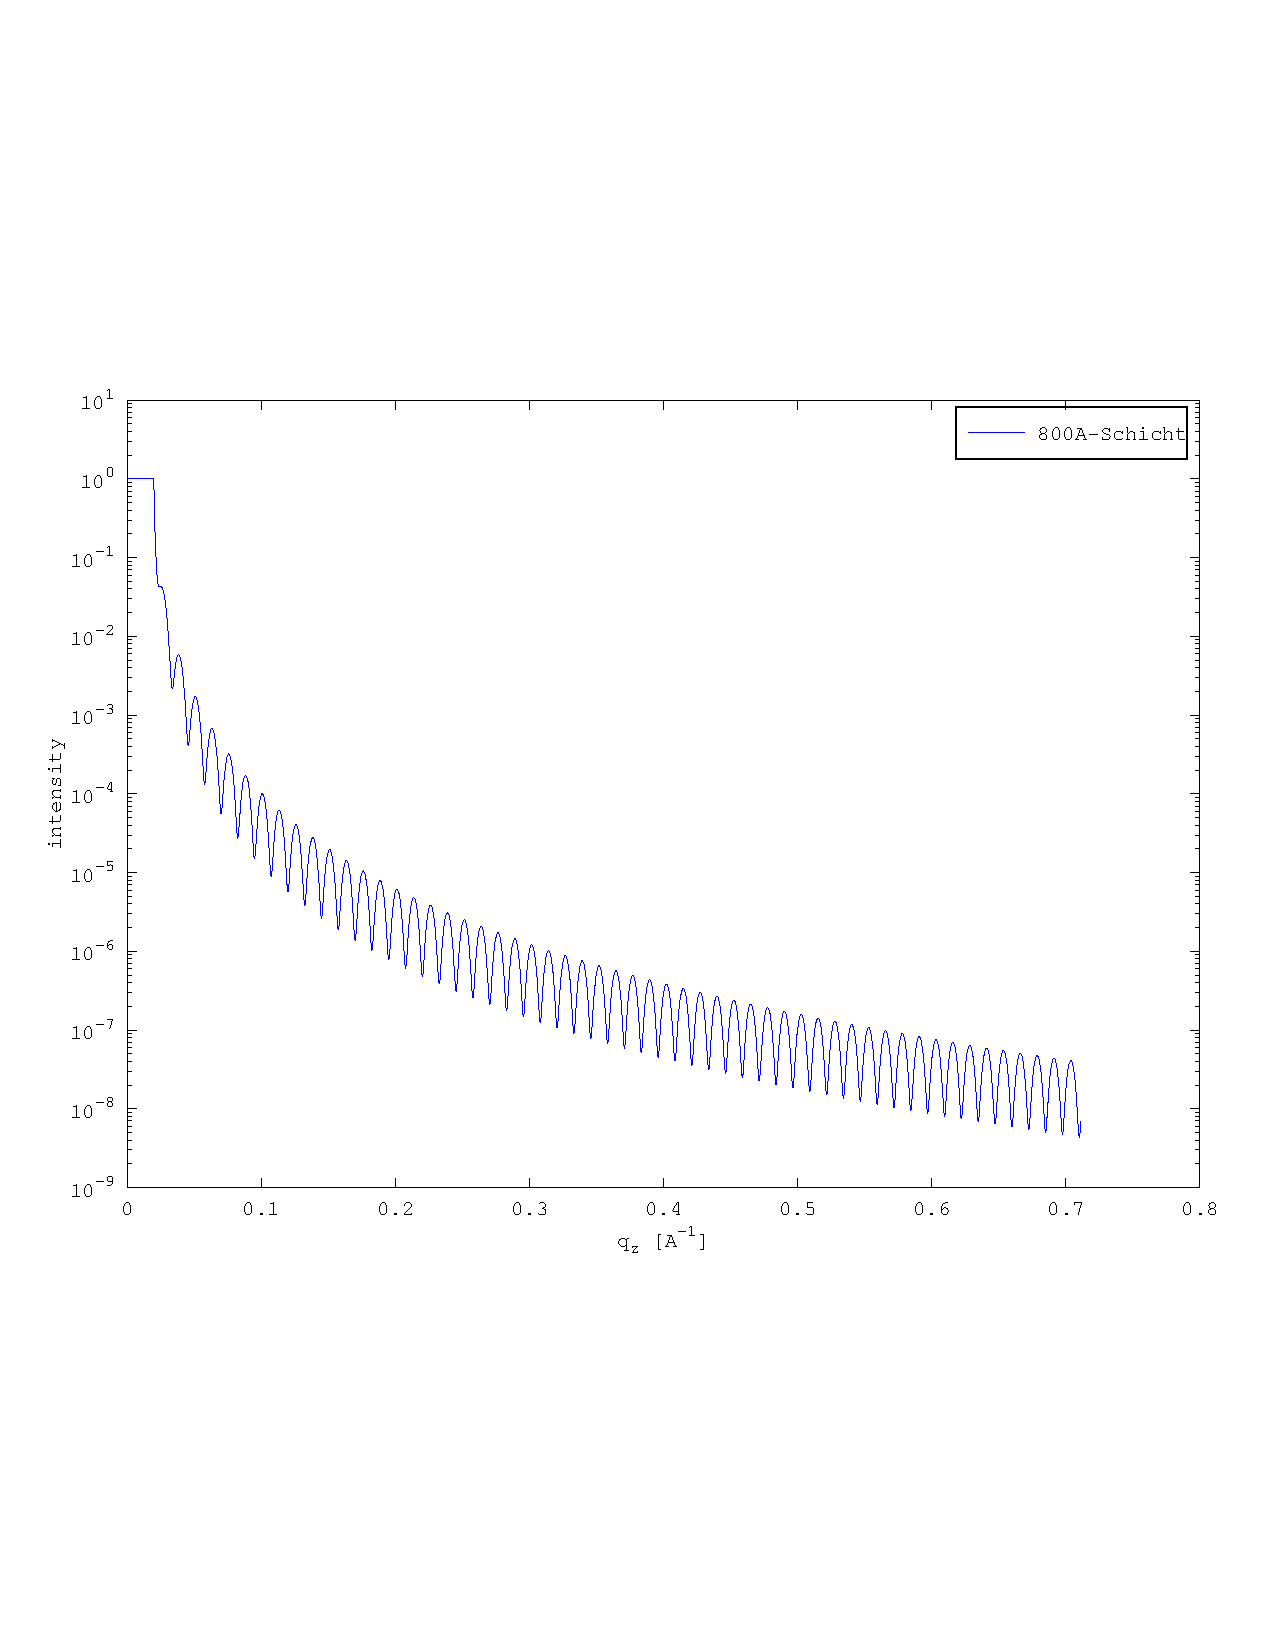
\includegraphics[width=0.9\textwidth]{images/reflektivitaet_schicht.pdf}
	\captionof{figure}{Durch  Parratt-Algorithmus berechnete Reflektivität für ein System mit einer Schicht mit $\delta=10^{-6}$ auf einem Substrat mit $\delta = 3\cdot 10^{-6} $ }
	\label{fig:reflexionbeispiel}
\end{center}
\subsection{Rauigkeit}
Reale Flächen sind nicht perfekt eben, sondern besitzen eine Rauigkeit.
Die Rauigkeit der j-ten Grenzfläche wird durch die root-mean-square-Rauigkeit
\begin{equation}
\sigma_\indx{j}^2=\int \left(z-z_\indx{j} \right)^2 P_\indx{j}\left(z\right)~\mathrm{d}z
\end{equation}
approximiert.
Dabei gibt $P_\indx{j}\left(z\right)$ die Wahrscheinlichkeit an, dass die j-te Grenzfläche bei einer Position im Intervall $\left[z_\indx{j}+ z, z_\indx{j}+ z+\mathrm{d}z \right]$ liegt.
Beim Parratt-Algorithmus kann die Rauigkeit berücksichtigt werden, indem modifizierte Fresnelkoeffizienten
\begin{align}
\tilde{r}_\indx{j,j+1}&=r_\indx{j,j+1}\exp\left( -2k_\indx{z,j}k_\indx{z,j+1}\sigma_\indx{j}^2 \right) \\
\tilde{t}_\indx{j,j+1}&=t_\indx{j,j+1}\exp\left( \frac{1}{2}\left(k_\indx{z,j}-k_\indx{z,j+1}\right)\sigma_\indx{j}^2 \right)
\end{align}
verwendet werden. In Abbildung \ref{fig:rauigkeitbeispiel} ist die Auswirkung der Rauigkeit an einen konkreten Beispiel dargestellt.

\begin{center}
	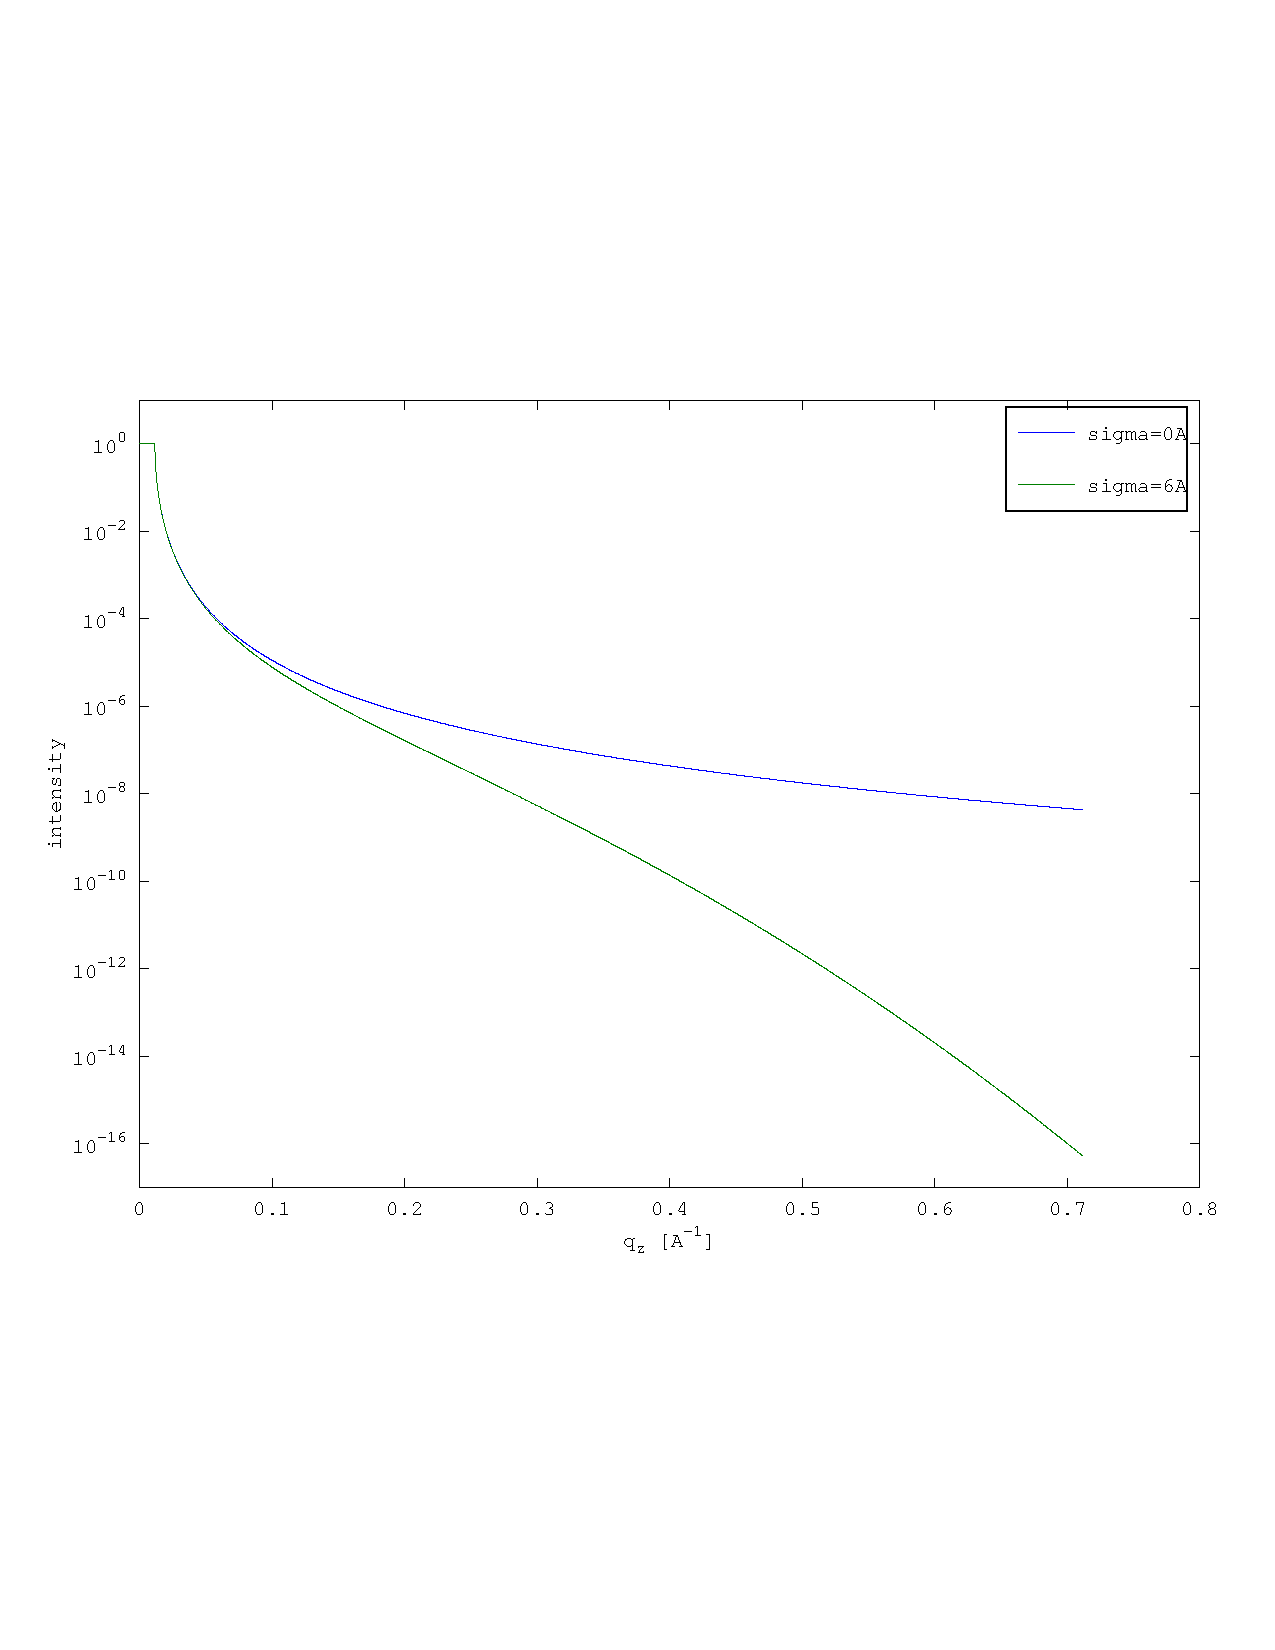
\includegraphics[width=0.9 \textwidth]{images/reflektivitaet_rau.pdf}
	\captionof{figure}{Berechnete Reflektivität für ein Substrat mit unterschiedlichen Rauigkeiten $\sigma_1=$\SI{0}{\angstrom} und $\sigma_2=$\SI{6}{\angstrom}.}
	\label{fig:rauigkeitbeispiel}
\end{center}
\subsection{Geometrischer Winkel}
Bei kleinen Winkeln trifft der Röntgenstrahl nicht vollständig auf die Probe. Der Winkel, ab dem der gesamte Strahl auf die Probe trifft, wird als Geometriewinkel 
\begin{align}
\alpha_{\indx{g}}=\arcsin \left( \frac{d_0}{D} \right)
\end{align}
bezeichnet. 
Dabei ist $D$ der Durchmesser der Probenoberfläche und $d_0$ die Höhe des Strahls.
Es lässt sich so ein Geometriefaktor 
\begin{align}
G=\left\lbrace\begin{matrix}
\frac{D \sin \alpha_{i} }{d} &,\ \alpha_{i} < \alpha_{\indx{g}} \\
1 &,\  \alpha_{i} > \alpha_{\indx{g}}
\end{matrix}\right.
\label{eq:geometriefaktor}
\end{align}
bestimmen, der angibt, welcher Anteil des Strahls auf die Probenoberfläche trifft.
Der Geometriefaktor muss reziprok mit der gemessenen Intensität multipliziert werden.

\section{Durchführung}
Der Versuch wurde am D8-Diffraktometer der Firma Bruker-AXS durchgeführt. Die im Diffraktometer erzeugte Röntgenstrahlung hat eine Wellenlänge von $\lambda=\SI{1.54}{\angstrom}$ \\ (Cu-K$_{\alpha}$-Linie) und wird von einer Kupferanodenröhre emittiert. Die emittierte divergente Strahlung wird von einem Göbelspiegel monochromatisiert und gebündelt. Nach dem Göbelspiegel wird die Strahlungsintensität durch einen Autoabsorber vermindert und der Strahl passiert eine Blende, die den Einfallswinkel $\alpha_i$ definiert. Dieser Aufbau ist in Abbildung \ref{fig:aufbau} dargestellt.
\begin{center}
	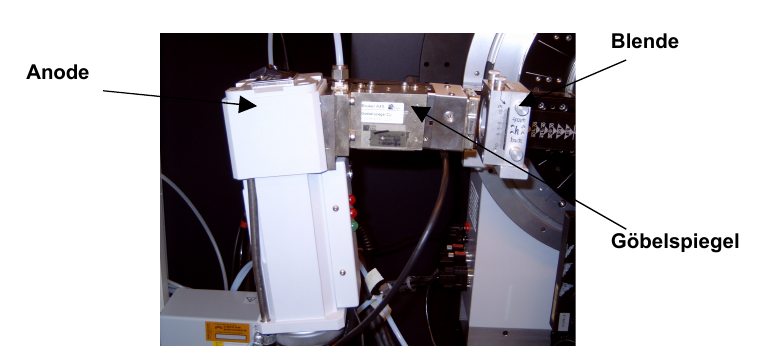
\includegraphics[width=0.8\textwidth]{images/aufbau.png}
	\captionof{figure}{Bild der Kupferanodenröhre mit Göbelspiegel und Blende}
	\label{fig:aufbau}
\end{center}
Nach der Reflexion wird Streustrahlung durch einen weiteren Spalt ausgefiltert. Eine weitere Blende legt den Ausfallwinkel $\alpha_f$ fest. \\

\subsection{Justage des D8-Labordiffraktometers}
Zur Justage des D8-Labordiffraktometers wird zunächst ein Detektorscan durchgeführt. Dabei bleibt die Röntgenröhre fest, während die Probe aus dem Strahl herausgefahren und die einfallende Intensität abhängig vom Winkel zwischen Röhre und Detektor gemessen wird. Ist ein Maximum zu erkennen, so wird der Scanbereich verkleinert, sodass das Maximum der Intensität sowie die Halbwertsbreite des entstehenden Signals genau bestimmt werden können. \\
Der nächste Schritt der Justage ist die Durchführung eines z-Scans, wobei eine halbe Abschattung durch die Probe erreicht werden soll. Dabei wird die Probe in den Strahl gefahren und die Intensität in Abhängigkeit von der Probenhöhe aufgenommen. Der Punkt der halben maximalen Intensität wird ausgewählt und als Probenhöhe festgelegt. \\
Als nächstes wird ein Rocking-Scan bei $2\Theta=0^{\circ}$ durchgeführt, wobei Detektor und Röhre um jeweils den gleichen Winkel um die Probe gedreht werden. Der erhaltene Scan hat eine Dreiecksform, wobei ein asymmetrisches Dreieck darauf hindeutet, dass die Probe sich nicht in der Mitte zwischen Röhre und Detektor befindet. Die Breite des Dreiecks wird für die Bestimmung des Geometriewinkels notiert. Detektor und Röhre werden an die Position des Maximums gefahren. \\
Zur präziseren Einstellung der Abschattung wird ein weiterer z-Scan gefahren und die Position der halben Abschattung eingestellt. Zur genaueren Justage des Strahlganges wird eine Rockingscan unter $2\Theta=0.3^{\circ}$ gefahren. Der Werte für Röhre und Detektor werden wieder für diesen Winkel übernommen. \\
Zur noch präziseren Abstimmung der halben Abschattung wird ein dritter z-Scan durchgeführt und so die endgültige Position der Probe im Strahl festgelegt. Danach wird ein weitere Rockingscan bei $2\Theta=1^{\circ}$ durchgeführt und wieder das Maximum abgespeichert. Die Justage wird mit einem weiteren Detektorscan und weiteren Rocking-Scans bei verschiedenen Werten für $2\Theta$ überprüft.

\subsection{Messung der Röntgenreflektivität}
Im Anschluss an die Justage wird ein Reflektivitätsscan an einer Polystyrolprobe, die sich auf einem Silizium-Wafer befindet, durchgeführt. Der Scanbereich geht dabei von $0^{\circ}$ bis $2.5^{\circ}$. \\
Mit einem "'diffusen Scan"' wird der Anteil der gestreuten Intensität bestimmt. Diese Messdaten werden nachher von den Messdaten der Primärmessung subtrahiert.

\section{Auswertung}

\subsection{Diffuser Scan und Geometriefaktor}
In Abbildung \ref{fig:diffus} sind der diffuse Scan, die Originalmessdaten und die bereinigten Daten dargestellt. Die weitere Datenverarbeitung wird mit den bereinigten Daten durchgeführt.
\begin{center}
	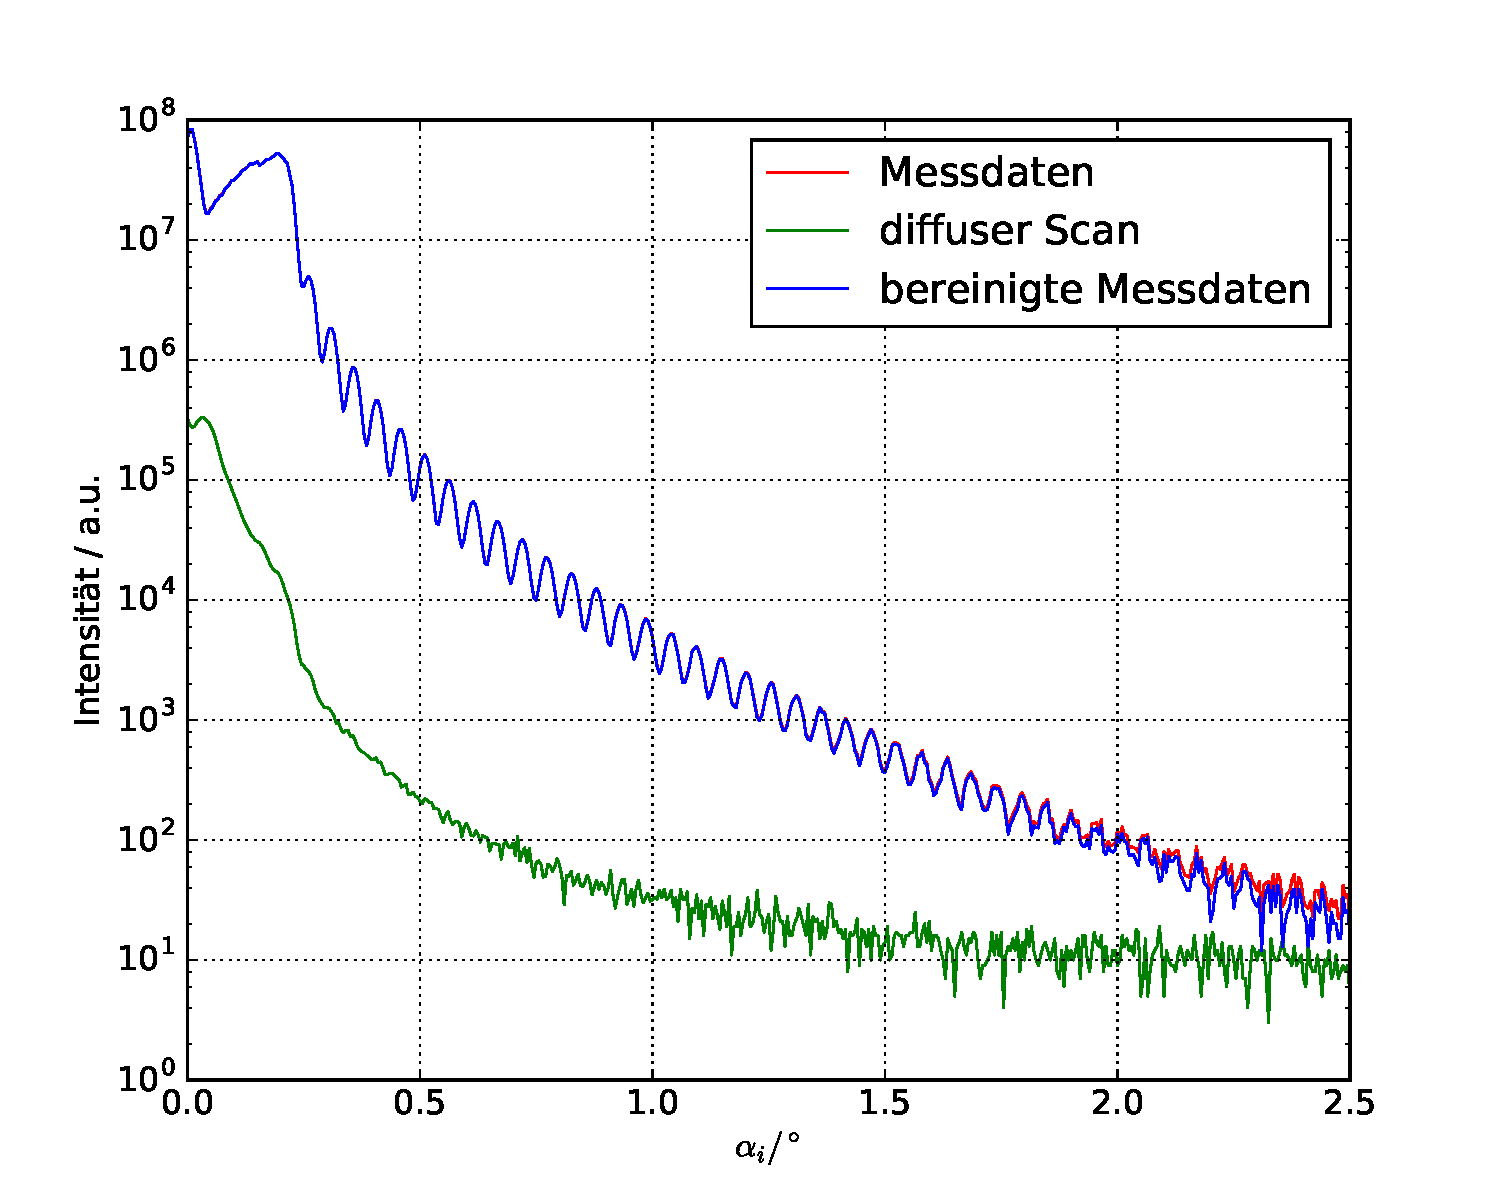
\includegraphics[width=0.8\textwidth]{images/rawdata.pdf}
	\captionof{figure}{Messwerte der Primär- und der Diffusmessung}
	\label{fig:diffus}
\end{center}
Der Geometriewinkel kann aus dem Rockingscan zu
\begin{align*}
\alpha_G=0.3247^{\circ}
\end{align*}
bestimmt werden. \\
Die Messdaten werden gemäß Gleichung \ref{eq:geometriefaktor} mit dem Geometriefaktor G korrigiert.

\subsection{Schichtdicke, Brechungsindex und Rauigkeit}
Aus dem korrigierten Signal werden die Minima bestimmt und die Distanz der einzelnen Minima zum jeweils nächsten Minima berechnet. Die entsprechenden Differenzen sind in Tabelle \ref{tab:minima} dargestellt, die Minima, die zur Mittelung verwendet worden sind, sind in Abbildung \ref{fig:reflektivitaet} dargestellt. \\
\begin{table}[H]
	\centering
	\captionof{table}{Minima und Distanz zum nächsten Minimum}
	\label{tab:minima}
	\begin{tabular}{r r}
		\toprule
		Minimum & Distanz / $^\circ$ \\
		\midrule
		1 & 0.05 \\
		2 & 0.05 \\
		3 & 0.05 \\
		4 & 0.055 \\
		5 & 0.05 \\
		6 & 0.055 \\
		7 & 0.05 \\
		8 & 0.05 \\
		9 & 0.055 \\
		10 & 0.055 \\
		11 & 0.055 \\
		12 & 0.05 \\
		13 & 0.055 \\
		14 & 0.05 \\
		15 & 0.06 \\
		16 & 0.05 \\
		17 & 0.055 \\
		18 & 0.055 \\
		19 & 0.05 \\
		20 & 0.055 \\
		21 & 0.05 \\
		\bottomrule
	\end{tabular}
\end{table}
Die Schichtdicke ergibt sich gemäß Formel \ref{eq:schichtdicke} zu
\begin{align*}
d=\SI{83.8(47)}{\nano \metre}\,.
\end{align*}
Zur Bestimmung der Rauigkeiten und der Brechungsindices wird mithilfe des Parratt-Algorithmus eine Theoriekurve berechnet, welche mithilfe von Python an die Messdaten angepasst wird. Dabei wird auch die Schichtdicke als Fitparameter verwendet. Die Fitparameter sind in Tabelle \ref{tab:fitparameter} dargestellt. Die Messdaten und die Theoriekurve sind in Abbildung \ref{fig:reflektivitaet} dargestellt.
\begin{table}[H]
	\centering
	\captionof{table}{Fitparameter}
	\label{tab:fitparameter}
	\begin{tabular}{r r}
		\toprule
		Fitparameter & Wert \\
		\midrule
		n$_{Schicht}$ & $1 - 25\cdot10^{-7} \pm 18\cdot10^{-7}$ \\
		n$_{Substrat}$ & $1 - 70\cdot10^{-7}\pm 0.4\cdot10^{-7}$ \\
		$\sigma_{Schicht}$ &  $\SI{0.75(1592)}{\nano\metre}$ \\
		$\sigma_{Substrat}$ & $\SI{0.35(1476)}{\nano\metre}$ \\
		$d$ & $\SI{83.8(119)}{\nano\metre}$ \\
		\bottomrule
	\end{tabular}
\end{table}

\begin{center}
	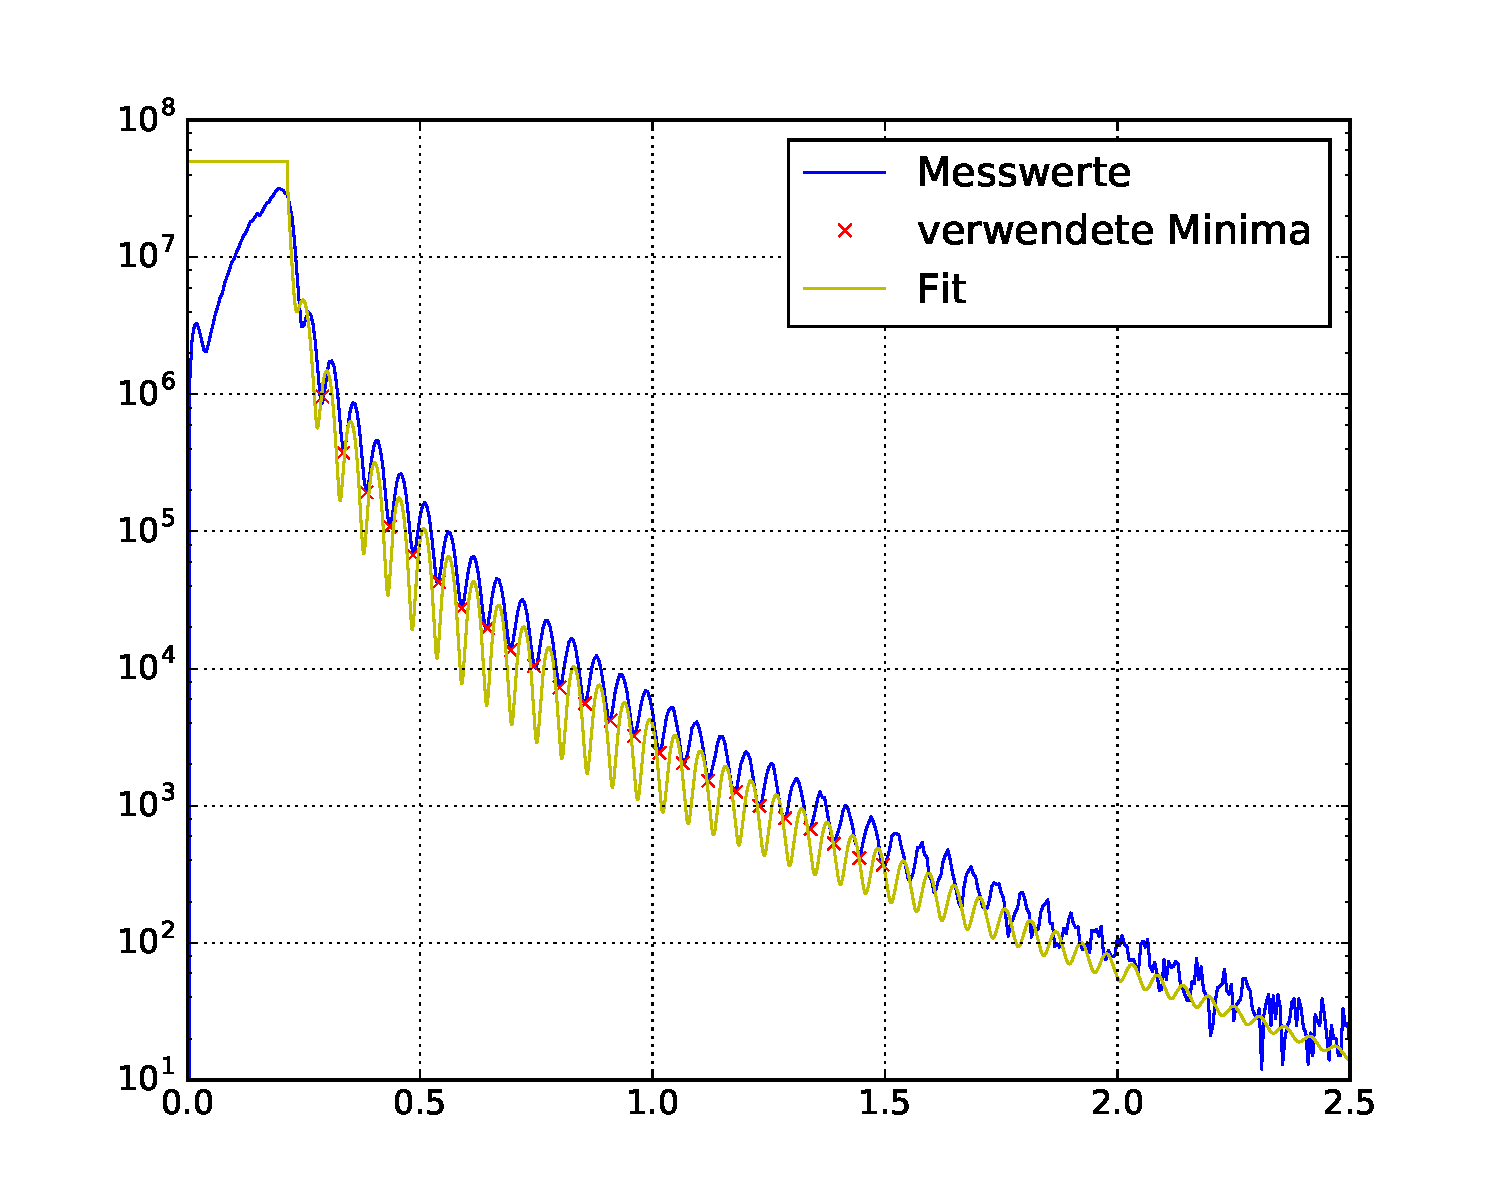
\includegraphics[width=0.8\textwidth]{images/reflectrometry.pdf}
	\captionof{figure}{Korrigiertes Messsignal, angepasste Theoriekurve und verwendete Peaks}
	\label{fig:reflektivitaet}
\end{center}

Mit Formel \ref{eq:elektronendichte} ergeben sich für die Elektronendichte von Schicht und Substrat
\begin{align*}
\rho_{\text{Schicht}}&=\SI{2.4(17)}{\cdot10^{29}\per\metre\cubed} \\
\rho_{\text{Substrat}}&=\SI{6.58(04)}{\cdot10^{29}\per\metre\cubed}\,.
\end{align*}

\section{Diskussion}
Bezüglich der Schichtdicke sind keine Literaturwerte bekannt, jedoch bewegt sich der Wert von $d=\SI{83.8(119)}{\nano \metre}$ in einer realistischen Größenordnung. \\
Der Brechungsindex der Polystyrolschicht weicht um 29\% vom Literaturwert\ref{q:anleitung} ab, der Brechungsindex des Substrats weicht nur um 7.8\% vom Literaturwert\ref{q:anleitung} ab. In beiden Fällen übersteigt die Abweichung die angegebene Unsicherheit, was auf die nicht perfekte Anpassung der Theoriekurve zurückzuführen ist. \\
Für die Werte der Rauigkeit liegen keine Literaturwerte vor, jedoch bewegen sich die Werte in einer realistischen Größenordnung. Die hohen statistischen Fehler liegen darin begründet, dass die Theoriekurve nicht genau mit den Messdaten in Übereinstimmung gebracht werden konnte. \\
Die Elektronendichten befinden sich in der richtigen Größenordnung, jedoch ergeben sich Abweichungen von 31\% bzw. 7\% von den Literaturwerten\ref{q:anleitung}, welche auf die Abweichungen der Brechungindices von den Literaturwerten zurückgehen.

\section{Quellen}
%\renewcommand{\labelenumi}{\value{enumi}}
\begin{enumerate}[label={[\arabic*]}]
\item \label{q:anleitung} \textbf{Physikalisches Praktikum}, TU Dortmund: \\
\textit{Versuchsanleitung zu Versuch: Röntgenreflektometrie} \\
\url{http://e1.physik.tu-dortmund.de/cms/Medienpool/Downloads/Roentgenreflektometrie_Versuch.pdf} (letzte Version vom 15.02.2017, 12:26)
\end{enumerate}

\end{document}